%!Tex Root=**/main.tex

\subsection{MonoGS}
\begin{Frame}{Framework}
	\begin{figure}[htbp]
		\centering
		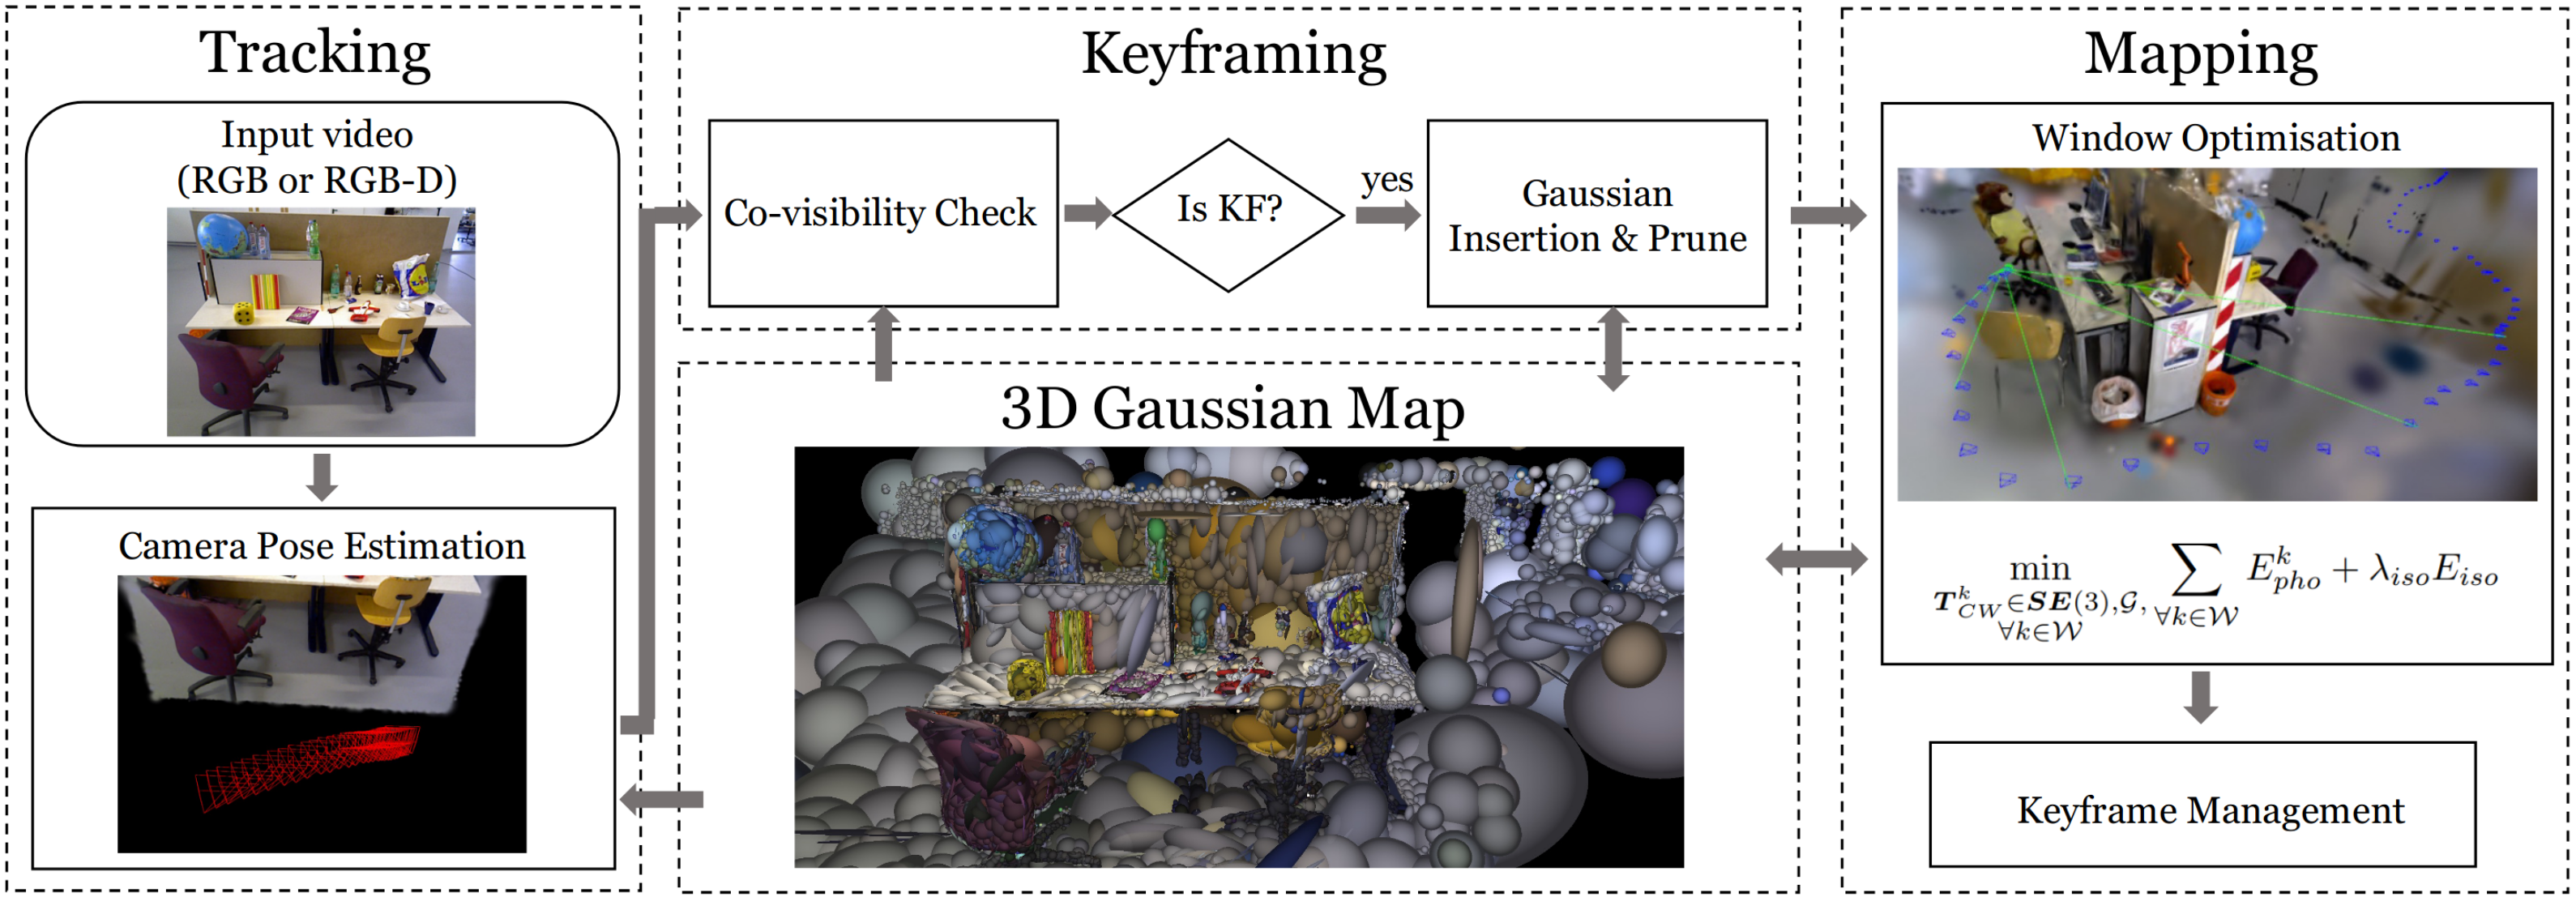
\includegraphics[width=\linewidth]{monogs/overview.png}
	\end{figure}
	\blfootnote{\href{http://arxiv.org/abs/2312.06741}{(CVPR Highlight, 2024) MonoGS: Gaussian Splatting SLAM}}
\end{Frame}

\tikzset{
	key/.style={
			draw=OrangeRed,
		},
	convention/.style={
			draw=Cerulean,
		},
	trick/.style={
			draw=ForestGreen,
		},
}

\begin{Frame}{Taxonomy of Methodology}
	\centering
	\resizebox{0.85\textwidth}{!}{
		\begin{forest}
			for tree={my tree}
			[
			MonoGS
				[
					Visual Odometry,for children={visible on=<1->}
						[
							Tracking,for children={visible on=<2->}
								[
									Inverse Rendering,for children={visible on=<3->}
										[
											Analytical Jacobians Derivation,key
										]
										[
											Photometric RGB \& Depth Loss,convention
										]
										[
											Optimizable Exposure,trick
										]
										[
											Penalization on non-edge/low-opacity pixels,trick
										]
								]
						]
						[
							Mapping,for children={visible on=<2->}
								[
									Bundle Adjustment,for children={visible on=<3->}
										[
											Photometric RGB \& Depth Loss,convention
										]
										[
											Isotropic Regularization,key
										]
										[
											Random Recall,trick
										]
								]
						]
				]
				[
					Online Pipeline,for children={visible on=<1->}
						[
							Keyframe Management,for children={visible on=<2->}
								[
									Registration,for children={visible on=<3->}
										[
											Gaussian Covisibility,key
										]
										[
											Relative Translation,convention
										]
								]
								[
									Removal,for children={visible on=<3->}
										[
											Gaussian Overlap Coefficient,key
										]
								]
						]
						[
							Gaussian Management,for children={visible on=<2->}
								[
									Insertion,for children={visible on=<3->}
										[
											Keyframing,convention
										]
								]
								[
									Pruning,for children={visible on=<3->}
										[
											Gaussian Covisibility,key
										]
								]
						]
				]
			]
		\end{forest}
	}
	\resizebox{0.08\textwidth}{!}{
		\begin{tikzpicture}[visible on=<3->]
			\node [my node for tree, draw=ForestGreen] (trick node) {trick};
			\node [my node for tree, draw=OrangeRed, above of = trick node] {key method};
			\node [my node for tree, draw=Cerulean, below of = trick node] (convention) {convention};
		\end{tikzpicture}
	}
	\blfootnote{\href{http://arxiv.org/abs/2312.06741}{(CVPR Highlight, 2024) MonoGS: Gaussian Splatting SLAM}}
\end{Frame}


\begin{Frame}{Tracking: Overview}
	\begin{figure}[htbp]
		\centering
		\resizebox{0.7\textwidth}{!}{
			\begin{forest} for tree={my tree}
				[
				Tracking
					[
						Inverse Rendering
							[
								Analytical Jacobians Derivation,key
							]
							[
								Photometric RGB \& Depth Loss,convention
							]
							[
								Optimizable Exposure,trick
							]
							[
								Penalization on non-edge/low-opacity pixels,trick
							]
					]
				]
			\end{forest}
		}
	\end{figure}
	\vspace*{\fill}
	\only<+->{\par Track camera poses by inverse rendering,}
	\vspace*{1.5ex}
	\begin{itemize}[<+->]
		\setlength{\itemsep}{1.5ex}
		\item \textcolor{OrangeRed}{through the extended differentiable rendering pipeline},
		\item \textcolor{Cerulean}{by a direct optimization against fixed 3D Gaussians,}
		\item \textcolor{ForestGreen}{with some tricks to be more adaptive to brightness and more robust to noise.}
	\end{itemize}
	\blfootnote{
		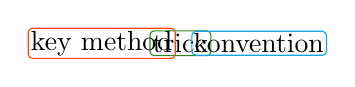
\begin{tikzpicture}
			\node [inner sep=1pt, rounded corners=1.5, draw=ForestGreen] (trick node) {trick};
			\node [inner sep=1pt, rounded corners=1.5, draw=OrangeRed, left of = trick node] {key method};
			\node [inner sep=1pt, rounded corners=1.5, draw=Cerulean, right of = trick node] (convention) {convention};
		\end{tikzpicture}
	}
	\blfootnote{\href{http://arxiv.org/abs/2312.06741}{(CVPR Highlight, 2024) MonoGS: Gaussian Splatting SLAM}}
\end{Frame}

\begin{Frame}{Tracking: Derivation of Jacobians \romannum{1}}
	\vspace*{-5em}
	\begin{overprint}[0.3\textheight]
		\only<1->{\par Firstly, let's review the \alert<1>{projection} of 3D Gaussians.}
		\begin{onlyenv}<2->
			\begin{equation}
				\mathcal{N}\left(\mu_w, \Sigma_w\right) \overset{\pi}{\mapsto} \mathcal{N}\left(\mu_i, \Sigma_i\right)
			\end{equation}
		\end{onlyenv}
		\only<3->{\par is achieved by}
	\end{overprint}
	\begin{figure}[htbp]
		\centering
		\begin{minipage}[c]{0.35\linewidth}
			\begin{onlyenv}<3->
				\resetcolorseries[4]{marknode-color-series}
				\resetcolorseries[4]{annotation-color-series}
				\begin{align}
					\alt<7->{\tikzmarknode{n3}{\colorbox{marknode-color-series!![3]}{\(\mu_{i}\)}}}{\mu_{i}}
					=
					\alt<6->{\tikzmarknode{n2}{\colorbox{marknode-color-series!![2]}{\(\pi\)}}}{\pi}
					\left(
					\alt<5->{\tikzmarknode{n1}{\colorbox{marknode-color-series!![1]}{\(\mathbf{T}_{cw}\)}}}{\mathbf{T}_{cw}}
					\cdot
					\alt<4->{\tikzmarknode{n0}{\colorbox{marknode-color-series!![0]}{\(\mu_{w}\)}}}{\mu_{w}}
					\right)
				\end{align}
				\begin{annotatedEquationEnv}
					\only<4->{\annotatedEquation{colorseries}{n0}{south}{0em}{-1em}{north west}{annotation-color-series}{\(\in \mathbb{P}^3\), 3D(world) mean}{east}}
					\only<5->{\annotatedEquation{colorseries}{n1}{south}{0em}{-3em}{north west}{annotation-color-series}{\(\in \mathrm{SE}(3)\), camera pose}{east}}
					\only<6->{\annotatedEquation{colorseries}{n2}{south}{0em}{-5em}{north west}{annotation-color-series}{projection}{east}}
					\only<7->{\annotatedEquation{colorseries}{n3}{south}{0}{-7em}{north west}{annotation-color-series}{\(\in \mathbb{P}^2\), 2D(image) mean}{east}}
				\end{annotatedEquationEnv}
			\end{onlyenv}
		\end{minipage}
		\begin{minipage}[c]{0.60\linewidth}
			\begin{onlyenv}<3->
				\resetcolorseries[4]{marknode-color-series}
				\resetcolorseries[4]{annotation-color-series}
				\begin{align}
					\alt<11->{\tikzmarknode{n3}{\colorbox{marknode-color-series!![3]}{\(\Sigma_{i}\)}}}{\Sigma_{i}}
					=
					\alt<10->{\tikzmarknode{n2}{\colorbox{marknode-color-series!![2]}{\(\mathbf{J}_{\pi}\)}}}{\mathbf{J}_{\pi}}
					\alt<9->{\tikzmarknode{n1}{\colorbox{marknode-color-series!![1]}{\(\mathbf{R}_{cw}\)}}}{\mathbf{R}_{cw}}
					\alt<8->{\tikzmarknode{n0}{\colorbox{marknode-color-series!![0]}{\(\Sigma_{w}\)}}}{\Sigma_{w}}  \mathbf{R}_{cw}^{\mathrm{T}} \mathbf{J}_{\pi}^{\mathrm{T}}
				\end{align}
				\begin{annotatedEquationEnv}
					\only<8->{\annotatedEquation{colorseries}{n0}{south}{0em}{-1em}{north west}{annotation-color-series}{\(\in \mathbb{R}^{3\times 3}\), 3D(world) covariance}{east}}
					\only<9->{\annotatedEquation{colorseries}{n1}{south}{0em}{-3em}{north west}{annotation-color-series}{\(\in \mathrm{SO(3)}\), rotation component of \(\mathbf{T}_{cw}\)}{east}}
					\only<10->{\annotatedEquation{colorseries}{n2}{south}{0em}{-5em}{north west}{annotation-color-series}{\(\in \mathbb{R}^{2\times 3}\), Jacobian of the linear approximation of \(\pi\)}{east}}
					\only<11->{\annotatedEquation{colorseries}{n3}{south}{0em}{-7em}{north west}{annotation-color-series}{\(\in \mathbb{R}^{2\times 2}\), 2D(image) covariance}{east}}
				\end{annotatedEquationEnv}
			\end{onlyenv}
		\end{minipage}
	\end{figure}
	\blfootnote{\href{http://arxiv.org/abs/2312.06741}{(CVPR Highlight, 2024) MonoGS: Gaussian Splatting SLAM}}
\end{Frame}

\begin{Frame}{Tracking: Derivation of Jacobians \romannum{2}}
	\par The chain rule,
	\begin{alignat}{1}
		\frac{\partial \mu_i}{\partial \mathbf{T}_{cw}}    & = \frac{\partial \mu_i}{\partial \mu_c} \frac{\partial \mu_c}{\partial \mathbf{T}_{cw}}                                                                                                                                                                               \\
		\frac{\partial \Sigma_i}{\partial \mathbf{T}_{cw}} & = \frac{\partial \Sigma_i}{\partial \mathbf{J}_{\pi}} \frac{\partial \mathbf{J}_{\pi}}{\partial \mu_c} \frac{\partial \mu_c}{\partial \mathbf{T}_{cw}} + \frac{\partial \Sigma_i}{\partial \mathbf{R}_{cw}} \frac{\partial \mathbf{R}_{cw}}{\partial \mathbf{T}_{cw}}
	\end{alignat}
	\pause
	\par The Lie Algebra,
	\begin{alignat}{1}
		\frac{\partial \mu_c}{\partial \mathbf{T}_{cw}}           & = \begin{bmatrix}
			                                                              \mathbf{I} & -\mu_{c}^{\times}
		                                                              \end{bmatrix}               \\
		\frac{\partial \mathbf{R}_{cw}}{\partial \mathbf{T}_{cw}} & = \begin{bmatrix}
			                                                              \mathbf{0} & - \mathbf{R}_{cw}^{\times}(:,1) \\
			                                                              \mathbf{0} & - \mathbf{R}_{cw}^{\times}(:,2) \\
			                                                              \mathbf{0} & - \mathbf{R}_{cw}^{\times}(:,3) \\
		                                                              \end{bmatrix}
	\end{alignat}
	\blfootnote{\href{http://arxiv.org/abs/2312.06741}{(CVPR Highlight, 2024) MonoGS: Gaussian Splatting SLAM}}
\end{Frame}

\begin{Frame}{Online Pipeline: Overview}
	\begin{figure}[htbp]
		\centering
		\resizebox{0.8\textwidth}{!}{
			\begin{forest}
				for tree={my tree}
				[
				Online Pipeline
					[
						Keyframe Management
							[
								Registration
									[
										Gaussian Covisibility,key
									]
									[
										Relative Translation,convention
									]
							]
							[
								Removal
									[
										Gaussian Overlap Coefficient,key
									]
							]
					]
					[
						Gaussian Management
							[
								Insertion
									[
										Keyframing,convention
									]
							]
							[
								Pruning
									[
										Gaussian Covisibility,key
									]
							]
					]
				]
			\end{forest}
		}
	\end{figure}
	\par \alert<+|handout:0>{Keyframe Management}:
	\vspace*{1.5ex}
	\begin{itemize}[<+->]
		\setlength{\itemsep}{1.5ex}
		\item \alert<.|handout:0>{Classic} strategies, e.g. covisibility \& overlap, from DSO~\autocite{engel2016dso}.
		\item \alert<.|handout:0>{Off-the-shelf} occlusion-aware Gaussian visibility is leveraged to construct metrics.
	\end{itemize}
	\blfootnote{
		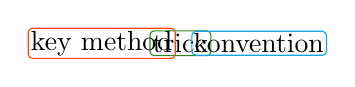
\begin{tikzpicture}
			\node [inner sep=1pt, rounded corners=1.5, draw=ForestGreen] (trick node) {trick};
			\node [inner sep=1pt, rounded corners=1.5, draw=OrangeRed, left of = trick node] {key method};
			\node [inner sep=1pt, rounded corners=1.5, draw=Cerulean, right of = trick node] (convention) {convention};
		\end{tikzpicture}
	}
	\blfootnote{\href{http://arxiv.org/abs/1607.02565}{(arXiv, 2016) DSO: Direct Sparse Odometry}}
	\blfootnote{\href{http://arxiv.org/abs/2312.06741}{(CVPR Highlight, 2024) MonoGS: Gaussian Splatting SLAM}}
\end{Frame}

\begin{Frame}{Online Pipeline: Overview}
	\begin{figure}[htbp]
		\centering
		\resizebox{0.8\textwidth}{!}{
			\begin{forest}
				for tree={my tree}
				[
				Online Pipeline
					[
						Keyframe Management
							[
								Registration
									[
										Gaussian Covisibility,key
									]
									[
										Relative Translation,convention
									]
							]
							[
								Removal
									[
										Gaussian Overlap Coefficient,key
									]
							]
					]
					[
						Gaussian Management
							[
								Insertion
									[
										Keyframing,convention
									]
							]
							[
								Pruning
									[
										Gaussian Covisibility,key
									]
							]
					]
				]
			\end{forest}
		}
	\end{figure}
	\par \alert<+|handout:0>{Gaussian Management:}
	\vspace*{1.5ex}
	\begin{itemize}[<+->]
		\setlength{\itemsep}{1.5ex}
		\item \alert<.>{Insertion:} triggered by \alert<.>{keyframing}, followed by \alert<.>{Gaussian initialization}.
		\item \alert<.>{Pruning:} to remove unstable/incorrect Gaussians by covisibility in a monocular setting.
	\end{itemize}
	\blfootnote{
		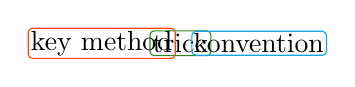
\begin{tikzpicture}
			\node [inner sep=1pt, rounded corners=1.5, draw=ForestGreen] (trick node) {trick};
			\node [inner sep=1pt, rounded corners=1.5, draw=OrangeRed, left of = trick node] {key method};
			\node [inner sep=1pt, rounded corners=1.5, draw=Cerulean, right of = trick node] (convention) {convention};
		\end{tikzpicture}
	}
	\blfootnote{\href{http://arxiv.org/abs/1607.02565}{(arXiv, 2016) DSO: Direct Sparse Odometry}}
	\blfootnote{\href{http://arxiv.org/abs/2312.06741}{(CVPR Highlight, 2024) MonoGS: Gaussian Splatting SLAM}}
\end{Frame}

\begin{Frame}{Keyframe Management: Prerequistes}
	\begin{enumerate}
		\setlength{\itemsep}{3ex}
		\item<+-> \alert<.>{What} is keyframing or keyframe management?
			\vspace*{1.5ex}
			\begin{itemize}
				\setlength{\itemsep}{1.5ex}
				\item<+-> A strategy of \alert<.>{selecting} and \alert<.>{utilizing} a \alert<.>{crucial subset} of frames.
			\end{itemize}
		\item<+-> \alert<.>{Why} do we need keyframing?
			\vspace*{1.5ex}
			\begin{itemize}
				\setlength{\itemsep}{1.5ex}
				\item<+-> \alert<.>{Infeasible} to optimize jointly on all frames online.
					\vspace*{1.5ex}
					\visible<+->{\par (a \alert<.>{trade-off} between efficiency and accuracy/robustness/...)}
			\end{itemize}
		\item<+-> \alert<.>{How} should we select keyframes?
			\vspace*{1.5ex}
			\begin{itemize}
				\setlength{\itemsep}{1.5ex}
				\item<+-> \alert<.>{non-redundant} and observing the \alert<.>{same area}.
				\item<+-> spanning a \alert<.>{wide baseline} for better multi-view constraints.
			\end{itemize}
	\end{enumerate}
	\blfootnote{\href{http://arxiv.org/abs/2312.06741}{(CVPR Highlight, 2024) MonoGS: Gaussian Splatting SLAM}}
\end{Frame}

\begin{Frame}{Keyframe Management: Registration \romannum{1}}
	\blfootnote{In practice, \(\sf \tau_{1} = 0.95\).}
	\blfootnote{\href{http://arxiv.org/abs/2312.06741}{(CVPR Highlight, 2024) MonoGS: Gaussian Splatting SLAM}}
	\begin{overprint}[\textheight]
		\par If \alert<+>{any} of the following conditions \alert<.>{is true}...
		\vspace*{\fill}
		\begin{block}<+->{\alert<.|handout:0>{Small Gaussian Covisibility}\hfill Condition \romannum{1}, Keyframe Registration}
			Gaussian covisibility between the current frame and the previous keyframe drops below a threshold.
			\begin{figure}[htbp]
				\centering
				\resetcolorseries[3]{marknode-color-series}
				\resetcolorseries[3]{annotation-color-series}
				\begin{align}
					\frac{\left\vert\operatorname{v}\left(\mathcal{G}, \mathcal{F}_{i}\right)
					\cap
					\alt<3->{\tikzmarknode{n0}{\colorbox{marknode-color-series!![0]}{\(\operatorname{v}\left(\mathcal{G}, \mathcal{F}_{j}\right)\)}}}{\operatorname{v}\left(\mathcal{G}, \mathcal{F}_{j}\right)}\right\vert}
					{\left\vert\operatorname{v}\left(\mathcal{G}, \alt<4->{\tikzmarknode{n1}{\colorbox{marknode-color-series!![1]}{\(\mathcal{F}_{i}\)}}}{\mathcal{F}_{i}}\right) \cup \operatorname{v}\left(\mathcal{G}, \alt<5->{\tikzmarknode{n2}{\colorbox{marknode-color-series!![2]}{\(\mathcal{F}_{j}\)}}}{\mathcal{F}_{j}}\right) \right\vert} < \tau_1
				\end{align}
				\begin{annotatedEquationEnv}
					\only<3->{\annotatedEquation{colorseries}{n0}{north}{0em}{1em}{south west}{annotation-color-series}{\(\subset \mathcal{G}\), \textbf{visible} Gaussians from frame \(j\)}{east}}
					\only<4->{\annotatedEquation{colorseries}{n1}{south}{0em}{-0.5em}{north east}{annotation-color-series}{the previous keyframe}{west}}
					\only<5->{\annotatedEquation{colorseries}{n2}{south}{0em}{-0.5em}{north west}{annotation-color-series}{the current frame}{east}}
				\end{annotatedEquationEnv}
			\end{figure}
		\end{block}
	\end{overprint}
\end{Frame}

\begin{Frame}{Keyframe Management: Registration \romannum{2}}
	\blfootnote{In practice, \(\sf \tau_{2}=0.04\). Additionally, evaluate the Gaussian covisibility only if the relative translation is not too small \((\sf > 0.02)\) for efficiency.}
	\blfootnote{\href{http://arxiv.org/abs/2312.06741}{(CVPR Highlight, 2024) MonoGS: Gaussian Splatting SLAM}}
	\begin{block}{\alert<1|handout:0>{Large Relative Translation}\hfill Condition \romannum{2}, Keyframe Registration}
		\par Translation from the previous keyframe w.r.t. to the median depth reaches a threshold.
		\begin{figure}[htbp]
			\centering
			\resetcolorseries[5]{marknode-color-series}
			\resetcolorseries[5]{annotation-color-series}
			\begin{align}
				\frac{ \left\Vert
				\alt<2->{\tikzmarknode{n0}{\colorbox{marknode-color-series!![0]}{\(\mathbf{t}_{\mathcal{F}_i \mathcal{F}_j}\)}}}{\mathbf{t}_{\mathcal{F}_i \mathcal{F}_j}}
				\right\Vert_2}
				{\alt<3->{\tikzmarknode{n1}{\colorbox{marknode-color-series!![1]}{\(\bar{D}_{\mathcal{F}_i \mathcal{F}_j}\)}}}{\bar{D}_{\mathcal{F}_i \mathcal{F}_j}}} > \tau_2
				, \quad
				\bar{D}_{\mathcal{F}_i \mathcal{F}_j}
				=
				\frac{1}{2
				\alt<5->{\tikzmarknode{n3}{\colorbox{marknode-color-series!![3]}{\(H\)}}}{H}
				\alt<6->{\tikzmarknode{n4}{\colorbox{marknode-color-series!![4]}{\(W\)}}}{W}
				}
				\sum^{\{\mathcal{F}_i,\mathcal{F}_j\}} \sum_{h=0}^{H} \sum_{w=0}^{W}
				\alt<4->{\tikzmarknode{n2}{\colorbox{marknode-color-series!![2]}{\(d(h,w)\)}}}{d(h,w)}
			\end{align}
			\begin{annotatedEquationEnv}
				\only<2->{\annotatedEquation{colorseries}{n0}{north}{0em}{0.5em}{south west}{annotation-color-series}{\(\in \mathbb{R}^3 \), translation from \(\mathcal{F}_i\) to \(\mathcal{F}_j\)}{east}}
				\only<3->{\annotatedEquation{colorseries}{n1}{south}{0em}{-0.5em}{north east}{annotation-color-series}{\(\in \mathbb{R} \), the median depth}{west}}
				\only<4->{\annotatedEquation{colorseries}{n2}{south}{0}{-0.5em}{north west}{annotation-color-series}{depth of pixel \((h,w)\)}{east}}
				\only<5->{\annotatedEquation{colorseries}{n3}{south}{0}{-0.5em}{north east}{annotation-color-series}{image height}{west}}
				\only<6->{\annotatedEquation{colorseries}{n4}{south}{0}{-0.5em}{north west}{annotation-color-series}{image width}{east}}
			\end{annotatedEquationEnv}
		\end{figure}
	\end{block}
\end{Frame}

\begin{Frame}{Keyframe Management: Removal \romannum{1}}
	\blfootnote{\href{http://arxiv.org/abs/2312.06741}{(CVPR Highlight, 2024) MonoGS: Gaussian Splatting SLAM}}
	\par If \alert<+>{any} of the following conditions \alert<.>{is true}...
	\vspace*{\fill}
	\begin{block}{\alert<.|handout:0>{Beyond Window Capacity}\hfill Condition \romannum{1}, Keyframe Removal}<+->
		Remove \alert<+|handout:0>{one} of previous keyframes \visible<+->{that \alert<.|handout:0>{minimize} the impact on the \alert<.|handout:0>{overall baseline length}.}
		\visible<+->{\begin{align}
				\mathcal{F}^{\ast} & = \underset{\mathcal{F}\in \mathcal{W}}{\arg\max}\;\operatorname{l}\Big(\mathcal{W}\;\backslash \big\{ \mathcal{F}\big\}\Big)
				\visible<+->{,\quad \operatorname{l}\left(\mathcal{W}\right) = \sum_{i=1}^{\left\vert \mathcal{W} \right\vert}\sum_{j=1}^{i} \left\Vert \mathbf{t}_{\mathcal{F}_i \mathcal{F}_j} \right\Vert }
			\end{align}}
		\visible<+->{\alert<.|handout:0>{\par Remark:} for the best multi-view constraints.}
	\end{block}
	\vspace*{\fill}
\end{Frame}

\begin{Frame}{Keyframe Management: Removal \romannum{2}}
	\begin{block}<+->{\alert<.|handout:0>{Low Gaussian Overlap Coefficient}\hfill Condition \romannum{2}, Keyframe Removal}
		Remove \alert<+|handout:0>{multiple} previous keyframes if the ``Gaussian overlap coefficient'' drops \alert<+>{below} a threshold.
		\visible<+->{
			\begin{equation}
				\frac{\vert \operatorname{v}\left(\mathcal{G}, \mathcal{F}_{i}\right) \cap \operatorname{v}\left(\mathcal{G}, \mathcal{F}_{j}\right) \vert}{\min \left(\vert\operatorname{v}\left(\mathcal{G}, \mathcal{F}_{i}\right) \vert, \vert\operatorname{v}\left(\mathcal{G}, \mathcal{F}_{j}\right) \vert\right)} < \tau_4
			\end{equation}
		}
		\visible<+->{\par \alert<.|handout:0>{Remark:} not observing the same area.}
	\end{block}
	\blfootnote{\href{https://en.wikipedia.org/wiki/Overlap_coefficient}{Szymkiewicz–Simpson coefficient}}
	\blfootnote{In practice, \(\sf \tau_{4} = 0.4.\)}
	\blfootnote{\href{http://arxiv.org/abs/2312.06741}{(CVPR Highlight, 2024) MonoGS: Gaussian Splatting SLAM}}
\end{Frame}

\begin{Frame}{Gaussian Management: Insertion}
	\begin{itemize}
		\setlength{\itemsep}{1.5ex}
		\item<+-> \alert<.>{Why} do we need ``Gaussian insertion''?
			\vspace*{1.5ex}
			\begin{itemize}
				\setlength{\itemsep}{1.5ex}
				\item<+-> \alert<.>{SLAM} is for robotic exploration.
			\end{itemize}
	\end{itemize}
	\vspace*{\fill}
	\begin{itemize}
		\setlength{\itemsep}{1.5ex}
		\item<+-> \alert<.>{When} do we need ``Gaussian insertion''?
	\end{itemize}
	\begin{block}{\alert<.|handout:0>{Keyframing}\hfill Condition \romannum{1}, Gaussian Insertion}<+->
		\par Insertion is triggered for every new keyframe.
	\end{block}
	\blfootnote{\href{http://arxiv.org/abs/2312.06741}{(CVPR Highlight, 2024) MonoGS: Gaussian Splatting SLAM}}
\end{Frame}

\begin{Frame}{Gaussian Management: Initialization}
	\begin{itemize}
		\setlength{\itemsep}{1.5ex}
		\item<+-> \alert<.>{How} do we insert Gaussians?
			\vspace*{1.5ex}
			\begin{itemize}
				\setlength{\itemsep}{1.5ex}
				\item<+-> Gaussian insertion is Gaussian \alert<.>{initialization}.
			\end{itemize}
	\end{itemize}
	\vspace*{\fill}
	\begin{block}{\alert<.|handout:0>{If Depth Available}\hfill Gaussian Initialization}<+->
		Back-project in a per-pixel, per-Gaussian approach.
	\end{block}
	\vspace*{\fill}
	\begin{block}{\alert<.|handout:0>{If Depth Unavailable}\hfill Gaussian Initialization}<+->
		Leverage the rendered depth map.
		\vspace*{1.5ex}
		\begin{itemize}[<+->]
			\setlength{\itemsep}{1.5ex}
			\item \alert<.|handout:0>{for pixels with depth:} use the rendered depth and assign a ``low'' covariance.
			\item \alert<.|handout:0>{for pixels w/o depth:} use the median of rendered depth and assign a ``high'' covariance.
		\end{itemize}
	\end{block}
	\blfootnote{
		In practice, ``low'': \(\sf 0.2 \sigma \); ``high'': \(0.5 \sigma\), where \(\sigma\) is the standard deviation of the rendered depth map.
	}
	\blfootnote{\href{http://arxiv.org/abs/2312.06741}{(CVPR Highlight, 2024) MonoGS: Gaussian Splatting SLAM}}
\end{Frame}

\begin{Frame}{Gaussian Management: Pruning}
	\begin{itemize}
		\setlength{\itemsep}{1.5ex}
		\item<+-> \alert<.>{Why} do we need ``Gaussian Pruning''?
			\vspace*{1.5ex}
			\begin{itemize}
				\setlength{\itemsep}{1.5ex}
				\item<+-> if depth \alert<.>{unavailable}, too many \alert<.>{incorrect} newly inserted Gaussians.
			\end{itemize}
	\end{itemize}
	\vspace*{\fill}
	\begin{block}{\alert<.|handout:0>{Low Gaussian Opacity} \hfill Condition \romannum{1}, Gaussian Pruning}<+->
		Low opacity Gaussians are pruned.
		\begin{equation}
			\{\mathcal{G}_i \in \mathcal{G}\;\vert\;\alpha(\mathcal{G}_i) < \tau_{\alpha} \}
		\end{equation}
	\end{block}
	\vspace*{\fill}
	\begin{block}{\alert<.|handout:0>{Low Gaussian Covisibility} \hfill Condition \romannum{2}, Gaussian Pruning}<+->
		For ``just'' inserted Gaussians but unobserved by ``some other'' keyframes, are pruned out.
	\end{block}
	\blfootnote{If no pruning, although the majority of incorrect Gaussians vanish quickly in following optimization, there are some survivals.}
	\blfootnote{In practice, \(\sf \tau_{\alpha}=0.7\).}
	\blfootnote{In practice, the pruned Gaussians are inserted in the last 3 keyframes and unobserved by any other 3 keyframes in the sliding window.}
	\blfootnote{\href{http://arxiv.org/abs/2312.06741}{(CVPR Highlight, 2024) MonoGS: Gaussian Splatting SLAM}}
\end{Frame}

\begin{Frame}{Mapping: Overview}
	\begin{center}
		\resizebox{!}{0.25\textheight}{
			\begin{forest}
				for tree={my tree}
				[
				Mapping
					[
						Bundle Adjustment
							[
								Photometric RGB \& Depth Loss,convention
							]
							[
								Isotropic Regularization,key
							]
							[
								Random Recall,trick
							]
					]
				]
			\end{forest}
		}
	\end{center}
	\pause
	\vspace*{\fill}
	\begin{itemize}
		\setlength{\itemsep}{1.5ex}
		\item<+-> \alert<.>{Why} do we need mapping in \textbf{3DGS} SLAM?
			\vspace*{1.5ex}
			\begin{itemize}
				\setlength{\itemsep}{1.5ex}
				\item<+-> \alert<.|handout:0>{Local}: Optimize newly inserted 3D Gaussians.
				\item<+-> \alert<.|handout:0>{Global}: Reconstruct a globally 3D-coherent structure.
			\end{itemize}
	\end{itemize}
	\blfootnote{
		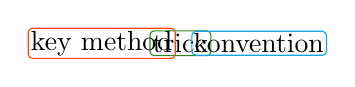
\begin{tikzpicture}
			\node [inner sep=1pt, rounded corners=1.5, draw=ForestGreen] (trick node) {trick};
			\node [inner sep=1pt, rounded corners=1.5, draw=OrangeRed, left of = trick node] {key method};
			\node [inner sep=1pt, rounded corners=1.5, draw=Cerulean, right of = trick node] (convention) {convention};
		\end{tikzpicture}
	}
	\blfootnote{\href{http://arxiv.org/abs/2312.06741}{(CVPR Highlight, 2024) MonoGS: Gaussian Splatting SLAM}}
\end{Frame}

\begin{Frame}{Mapping: Bundle Adjustment \& Random Recall}
	\begin{block}<1->{\alert<1|handout:0>{Bundle Adjustment}}
		\vspace*{-1.5em}
		\begin{figure}[htbp]
			\centering
			\resetcolorseries[4]{marknode-color-series}
			\resetcolorseries[4]{annotation-color-series}
			\begin{equation}
				\underset{
				\alt<2->{\tikzmarknode{n0}{\colorbox{marknode-color-series!![0]}{\scriptsize \(\mathcal{G}\)}}}{\mathcal{G}},
				\alt<3->{\tikzmarknode{n1}{\colorbox{marknode-color-series!![1]}{\scriptsize \(\{\mathbf{T}_{cw}({\mathcal{F}_k})\vert \mathcal{F}_k\in \mathcal{W}\}\)}}}{\{\mathbf{T}_{cw}({\mathcal{F}_k})\vert \mathcal{F}_k\in \mathcal{W}\}}
				}{
				\operatorname{argmin}
				}
				\sum_{\mathcal{F}_k}^{
					\mathcal{W}
				}
				\mathcal{L}_{pho}\left({\mathcal{F}_k}\right)
			\end{equation}
			\begin{annotatedEquationEnv}
				\only<2->{\annotatedEquation{colorseries}{n0}{south}{0em}{-0.5em}{north east}{annotation-color-series}{3D Gaussians}{west}}
				\only<3->{\annotatedEquation{colorseries}{n1}{south}{0em}{-0.5em}{north west}{annotation-color-series}{camera poses of keyframes in the sliding window}{east}}
			\end{annotatedEquationEnv}
		\end{figure}
	\end{block}
	\vspace*{\fill}
	\begin{block}<4->{\alert<4|handout:0>{Random Recall}}
		\par Besides \(\mathcal{W}\), ``some'' randomly selected historical keyframes are also leveraged in BA to avoid forgetting the global map.
	\end{block}
	\blfootnote{\href{http://arxiv.org/abs/2312.06741}{(CVPR Highlight, 2024) MonoGS: Gaussian Splatting SLAM}}
\end{Frame}

\begin{Frame}{Mapping: Isotropic Regularization}
	\begin{itemize}[<+->]
		\setlength{\itemsep}{1.5ex}
		\item \alert<.>{Why} do we need ``isotropic regularization''?
		      \vspace*{1.5ex}
		      \begin{itemize}
			      \setlength{\itemsep}{1.5ex}
			      \item \alert<.|handout:0>{Observation:} isotropic Gaussians behave better than anisotrophic.
			      \item \alert<.|handout:0>{Analysis:} no constraints on the elongation along the viewing ray direction, \textbf{even with depth}.
		      \end{itemize}
	\end{itemize}
	\vspace*{\fill}
	\begin{block}<4->{\alert<.|handout:0>{Isotropic Regularization}}
		\vspace*{1em}
		\begin{figure}[htbp]
			\resetcolorseries[4]{marknode-color-series}
			\resetcolorseries[4]{annotation-color-series}
			\centering
			\begin{equation}
				\mathcal{L}_{iso} = \sum_{i=1}^{
				\alt<5->{\tikzmarknode{n0}{\colorbox{marknode-color-series!![0]}{\scriptsize \(\vert \mathcal{G} \vert\)}}}{\vert \mathcal{G} \vert}
				}
				\Vert
				\alt<6->{\tikzmarknode{n1}{\colorbox{marknode-color-series!![1]}{\(\mathbf{s}(\mathcal{G}_i)\)}}}{\mathbf{s}(\mathcal{G}_i)}
				-
				\alt<7->{\tikzmarknode{n2}{\colorbox{marknode-color-series!![2]}{\(\bar{\mathbf{s}}(\mathcal{G}_i)\)}}}{\bar{\mathbf{s}}(\mathcal{G}_i)}
				\Vert_1
				,\quad
				\visible<7->{\bar{\mathbf{s}}(\mathcal{G}_i) = \begin{bmatrix}
						\left( s(\mathcal{G}_i)^{x} + s(\mathcal{G}_i)^{y} + s(\mathcal{G}_i)^{z} \right) / 3 \\
						\left( s(\mathcal{G}_i)^{x} + s(\mathcal{G}_i)^{y} + s(\mathcal{G}_i)^{z} \right) / 3 \\
						\left( s(\mathcal{G}_i)^{x} + s(\mathcal{G}_i)^{y} + s(\mathcal{G}_i)^{z} \right) / 3 \\
					\end{bmatrix}}
			\end{equation}
			\begin{annotatedEquationEnv}
				\only<5->{\annotatedEquation{colorseries}{n0}{north}{0em}{3em}{south west}{annotation-color-series}{\(\in \mathbb{N}\), total number of Gaussians}{east}}
				\only<6->{\annotatedEquation{colorseries}{n1}{north}{0em}{3em}{south west}{annotation-color-series}{\(\in \mathbb{R}^3\), scale of \(i\)-th Gaussian}{east}}
				\only<7->{\annotatedEquation{colorseries}{n2}{north}{0em}{1.5em}{south west}{annotation-color-series}{\(\in \mathbb{R}^3\), averaged scale of \(i\)-th Gaussian}{east}}
			\end{annotatedEquationEnv}
		\end{figure}
	\end{block}
	\blfootnote{\href{http://arxiv.org/abs/2312.06741}{(CVPR Highlight, 2024) MonoGS: Gaussian Splatting SLAM}}
\end{Frame}

\begin{Frame}{Mapping: Conclusion}
	\begin{block}{Overall Optimization for Mapping}
		\begin{equation}
			\underset{\mathcal{G}, \{\mathbf{T}_{cw}({\mathcal{F}_k})\vert \mathcal{F}_k\in \mathcal{W}^{+}\}}{\operatorname{argmin}} \sum_{\mathcal{F}_k}^{\mathcal{W}^{+}} \mathcal{L}_{pho}\left({\mathcal{F}_k}\right) + \lambda_{iso} \mathcal{L}_{iso}
		\end{equation}
	\end{block}
	\blfootnote{\href{http://arxiv.org/abs/2312.06741}{(CVPR Highlight, 2024) MonoGS: Gaussian Splatting SLAM}}
\end{Frame}
